\chapter{Analyse et spécification des besoins}

\section*{Introduction}
\addcontentsline{toc}{section}{Introduction }
    \par {\huge L}a réussite de toute étude dépend de la qualité de la phase de démarrage. 
    De ce fait, l'étape d'analyse des besoins constitue la base de départ de notre travail 
    ainsi qu'une étape déterminante pour la suite. 
    Dans ce chapitre, nous évoquerons tout d'abord les besoins fonctionnels et non
    fonctionnels de notre solution. Ensuite Nous définissons clairement le flux de travail 
    qu'oon va élaborer tout au long de ce projet. Finalement, nous allons dresser le backlog produit qui contient toutes les fonctionnalités que nous
    allons utiliser comme étant la base essentielle de la phases suivantes de planification et de développement.
    \section{Concepts de base}

    Dans cette section, nous définissons et expliquons les principaux concepts et technologies essentiels à notre projet de monitoring des opérations sur Snowflake. La compréhension de ces concepts est cruciale pour saisir le fonctionnement et les objectifs de notre solution.
    
    \subsection{La platforme Snowflake }
    
    \textbf{Snowflake} est une plateforme de data warehousing cloud conçue pour le stockage et l'analyse de données à grande échelle.
    Elle offre des capacités de traitement massivement parallèle, permettant une scalabilité pratiquement illimitée. 
    Snowflake se distingue par la séparation des couches de stockage et de calcul, offrant ainsi des avantages en termes de flexibilité, de performance et de coût \cite{snowflake}.
    
    \textbf{Fonctionnalités clés de Snowflake :}
    \begin{itemize}
        \item \textit{Stockage des données} : Utilisation de la compression et de la partition pour optimiser le stockage ;
        \item \textit{Calcul élastique} : Possibilité de redimensionner les ressources de calcul en fonction des besoins ;
        \item \textit{Partage sécurisé des données} : Facilite le partage des données entre différentes organisations tout en assurant la sécurité ;
        \item \textit{Support SQL complet} : Prise en charge des commandes SQL standards pour la manipulation des données.
    \end{itemize}
    
    \subsection{Directed Acyclic Graph (DAG)}
    
    Un \textbf{DAG (Directed Acyclic Graph)} est une structure de données qui représente un ensemble de tâches et leurs dépendances sous forme
     de graphe dirigé sans cycles\cite{dagdef}. Dans le contexte des pipelines de données, un DAG est souvent utilisé pour définir les étapes de traitement des données et leur ordre d'exécution.
    
    \textbf{Utilisation des DAGs :}
    \begin{itemize}
        \item \textit{Planification des tâches} : Détermination de l'ordre dans lequel les tâches doivent être exécutées ; 
        \item \textit{Gestion des dépendances} : Assure que les tâches dépendantes sont exécutées dans le bon ordre ;
        \item \textit{Parallélisme} : Permet l'exécution simultanée de tâches indépendantes.
    \end{itemize}
    
    \subsection{Solution de Monitoring}
    
    Une \textbf{solution de monitoring} est un ensemble d'outils et de pratiques conçus pour surveiller les performances,
     la disponibilité et la santé des systèmes informatiques. Elle collecte, analyse et affiche des métriques et des logs 
     pour aider les administrateurs à détecter et résoudre les problèmes\cite{monitoring}.
    
    \textbf{Caractéristiques d'une solution de monitoring efficace :}
    \begin{itemize}
        \item \textit{Collecte de métriques en temps réel} : Surveillance continue des performances et des ressources ;
        \item \textit{Alertes et notifications} : Système d'alerte en cas d'anomalies ou de dépassement de seuils définis ;
        \item \textit{Visualisation des données} : Tableaux de bord interactifs pour l'analyse des métriques et des tendances ;
        \item \textit{Reporting} : Génération de rapports détaillés pour le suivi et l'analyse historique.
    \end{itemize}
    
    \subsection{Analyse des Données}
    
    L'\textbf{analyse des données} est la science qui consiste à examiner les données pour en tirer des informations permettant de prendre des décisions ou d'approfondir les connaissances sur divers sujets \cite{analyse}. Elle vise à comprendre et exploiter les données pour des prises de décision éclairées.
    
    \textbf{Étapes de l'analyse des données :}
    \begin{itemize}
        \item \textit{Collecte des données} : Réunir les données pertinentes à partir de diverses sources.
        \item \textit{Préparation des données} : Nettoyage et transformation des données brutes en un format utilisable.
        \item \textit{Modélisation} : Utilisation de modèles statistiques et algorithmiques pour analyser les données.
        \item \textit{Interprétation et visualisation} : Présentation des résultats sous forme de graphiques et de rapports compréhensibles.
    \end{itemize}
    
    \subsection{L'ingénierie des données}
    
    L'\textbf{ingénierie des données} est la discipline consistant à concevoir, construire et maintenir des systèmes et des architectures pour collecter, stocker et analyser des données. Elle se concentre sur la création de l'infrastructure permettant l'exploitation des données par les analystes pour des prises de décision éclairées.
    
    \textbf{Responsabilités du l'ingénierie des données :}
    \begin{itemize}
        \item \textit{Conception de pipelines de données} : Définir et implémenter les processus de collecte, de transformation et de stockage des données.
        \item \textit{Gestion des bases de données} : Assurer la performance, la sécurité et l'intégrité des bases de données.
        \item \textit{Optimisation des requêtes} : Améliorer les requêtes pour une exécution plus rapide et efficace.
        \item \textit{Intégration de données} : Combiner les données provenant de diverses sources pour une vue unifiée.
    \end{itemize}
    
    Cette section vise à établir une compréhension claire des concepts et des technologies essentiels utilisés dans notre projet. Cela permettra de mieux appréhender les choix de conception et les décisions techniques prises tout au long du développement de la solution de monitoring des opérations sur Snowflake.
    
\section{Capture des besoins}
\par La capture des besoins est une phase fondamentale dans la réalisation du projet puisque elle doit
permettre aux utilisateurs finaux et au maître d'ouvrage de bien exprimer leurs besoins et de bien
comprendre les fonctionnalités que le système va fournir.
    % Une sous section
    \subsection{Besoins fonctionnels}
        \par Cette section décrit en détail les besoins fonctionnels du projet de monitoring des opérations Snowflake.
        Ces besoins ont été identifiés à partir des exigences de l'entreprise et des utilisateurs, et sont essentiels pour le développement d'une solution efficace et adaptée aux besoins de l'entreprise.
    \begin{itemize}
            \item \textbf{La collecte automatique des données de Snowflake} :
            Le système doit être capable de collecter automatiquement les données de Snowflake, y compris les requêtes exécutées et leurs informations, l'utilisation des ressources (CPU, mémoire, stockage), les bases de données et leurs objets ( tâches, tables, tubes, etc. ), les statistiques sur les entrepôts de données, etc... ;
            
            \item \textbf{La surveillance en temps réel des requêtes SQL} :
            Le système doit surveiller en temps réel les requêtes SQL exécutées sur Snowflake, enregistrant ces informations détaillées, les erreurs éventuelles, et en identifiant les requêtes lentes ou mal optimisées ;
            
            \item \textbf{La surveillance en temps réel des entrepôts de données} :
            Le système doit surveiller en temps réel les métriques des entrepôts de données, y compris l'utilisation de l'espace disque, la répartition de la charge de travail et la consommation de ressources ;
            
            \item \textbf{L'élaboration des tableaux de bord interactifs pour les métriques clés} :
            Le système doit fournir des tableaux de bord interactifs permettant de visualiser les métriques clés de performance de Snowflake, y compris les temps de réponse des requêtes, l'utilisation des ressources et les statistiques sur les entrepôts de données ;
            
            \item \textbf{Suivi des tâches et leurs DAGs} :
            Le système doit permettre le suivi des tâches et des DAGs exécutées dans Snowflake, enregistrant les étapes effectuées, les tous leurs informations et les erreurs éventuelles ;
            
            \item \textbf{La surveillance de l'utilisation des crédits} :
            Le système doit surveiller l'utilisation des crédits de calcul sur Snowflake, enregistrant les crédits utilisés par chaque requête ou chaque tâche, ainsi que les tendances d'utilisation au fil du temps ;
            
            \item \textbf{La surveillance des utilisateurs et des accès} :
            Le système doit suivre l'activité des utilisateurs sur Snowflake, en enregistrant leurs requêtes exécutées, les objets accédées et les autorisations utilisées ;
            
            \item \textbf{Alertes et notifications en cas d'anomalies} :
            Le système doit générer des alertes et des notifications en temps réel en cas d'anomalies ou de situations critiques, telles qu'une augmentation soudaine du temps de réponse des requêtes ou une utilisation anormale des ressources; 
            
            \item \textbf{Personnalisation des tableaux de bord} :
            Le système doit permettre aux utilisateurs de personnaliser les tableaux de bord en fonction de leurs besoins spécifiques, en sélectionnant les métriques à afficher et en configurant les seuils d'alerte.
        \end{itemize}        
    % Une deuxième sous section
    \subsection{Besoins non fonctionnels}
  \par Cette section détaille les besoins non fonctionnels du projet de monitoring des opérations Snowflake. 
  Ces besoins concernent principalement les aspects de performance, de sécurité, d'évolutivité et d'expérience utilisateur de la solution. 
  Ils sont essentiels pour garantir que le système répond aux attentes de l'entreprise en termes de qualité et de fiabilité.

  \begin{itemize}
        \item\textbf{Besoins en Performance}

                \begin{enumerate}
                    \item[1.] \textbf{Temps de réponse} : Le système doit fournir des temps de réponse rapides pour l'affichage des tableaux de bord, afin de garantir une expérience utilisateur fluide ;
                    
                    \item[2.] \textbf{Évolutivité} : Le système doit être capable de gérer une grande quantité de données et de trafic sans compromettre ses performances, en s'adaptant de manière transparente à l'augmentation de la charge.
                \end{enumerate}
    
        \item\textbf{Besoins en Sécurité}
    
                \begin{enumerate}
                    \item[1.] \textbf{Confidentialité des données} : Le système doit garantir la confidentialité des données collectées, en assurant leur cryptage lors du stockage et de la transmission ;
                    
                    \item[2.] \textbf{Authentification et autorisation} : Le système doit mettre en place des mécanismes d'authentification robustes pour vérifier l'identité des utilisateurs 
                    et des administrateurs, ainsi que des contrôles d'autorisation pour limiter l'accès aux données sensibles.
                \end{enumerate}
    
        \item\textbf{Besoins en Disponibilité}
    
                \begin{enumerate}
                    \item[1.] \textbf{Disponibilité} : Le système doit être disponible en permanence, avec un temps de fonctionnement maximal et une reprise rapide en cas de panne ;
                    
                    \item[2.] \textbf{Tolérance aux pannes} : Le système doit être capable de résister aux pannes matérielles ou logicielles, en assurant la redondance des composants critiques et la sauvegarde des données.
                \end{enumerate}
    
        \item\textbf{Besoins en Expérience Utilisateur}
    
                \begin{enumerate}
                    \item[1.] \textbf{Facilité d'utilisation} : Le système doit être intuitif et convivial, avec une interface utilisateur bien conçue et une navigation facile ;
                    
                    \item[2.] \textbf{Personnalisation} : Le système doit permettre aux utilisateurs de personnaliser leur expérience, en configurant les préférences d'affichage et les paramètres de notification.
                \end{enumerate}
        \item \textbf{Archivage des données: }Les données historiques doivent être archivées de manière efficace pour garantir l'intégrité des données.
  \end{itemize}
  \section{Flux de travail}
  
  \par Durant la réalisation de notre projet, ce processus a été notre fil conducteur, nous permettantpermettons de passer par plusieurs étapes clés pour atteindre notre objectif. La figure \textbf{\ref{fig:BPMN}} suivante illustre notre processus métier :
    %code image
        \begin{figure}[H]
        \centering
        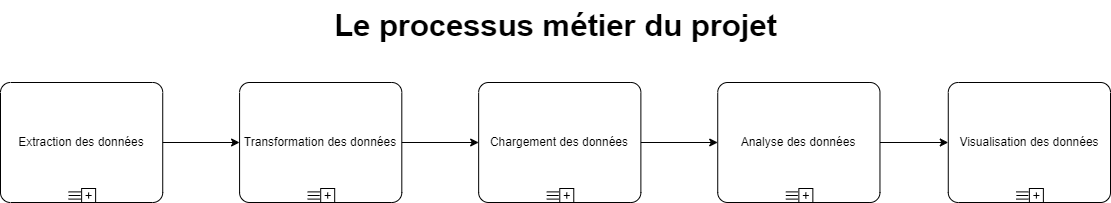
\includegraphics[width=1\linewidth, height=3.5cm]{img/conception/BPMN.png}
        \caption{Processus métier du projet}
        \label{fig:BPMN}
        \end{figure}
    %fin
  \par Maintenant, nous allons explorer en détail le flux de travail que nous avons suivi, en soulignant l'importance de chaque étape et en expliquant comment elles se sont complétées pour aboutir à une solution complète. Ensuite, nous examinerons chaque étape de manière approfondie pour comprendre comment elles ont contribué à notre succès global.
  \par Passons maintenant à l'examen détaillé de chacune de ces étapes.

  \begin{itemize}
  
  \item \textbf{Extraction des données :}
  \par Cette étape consistait à recueillir des informations provenant des différentes vues du système Snowflake. 
  L'objectif principal est de collecter les données nécessaires à notre analyse. 
  L'extraction de données est une phase cruciale dans l'ingénierie des données, car elle constitue le point de départ de tout projet d'analyse. 
  Les techniques d'extraction comprenaient des requêtes SQL avancées et l'automatisation des processus d'extraction pour garantir une collecte fiable et régulière.

  \item \textbf{Transformation des données :}
  \par L'objectif principal de cette étape est de nettoyer et structurer les données. Car, ces données brutes pouvaient contenir des erreurs, des doublons, des incohérences et/ou des valeurs manquantes. 
  Nous allons appliquer des techniques de nettoyage, telles que l'imputation des valeurs manquantes, la déduplication et la normalisation des données.
   De plus, des processus de transformation ont été utilisés pour convertir les données dans des formats appropriés pour l'étape suivante.

  \item \textbf{Chargement des données :}
  \par Une fois les données nettoyées et préparées, elles sont acheminées vers une base de données ou un entrepôt de données. Le chargement vise à stocker les données de manière centralisée pour une accessibilité et une analyse ultérieures.
   Cette phase garantit que les données sont correctement indexées, partitionnées et optimisées pour des requêtes rapides et efficaces.

  \item \textbf{Analyse des données :}
  \par Cette phase consiste à explorer les données pour en extraire des informations significatives. 
  L'analyse des données utilise des méthodes statistiques, des techniques de modélisation, des calculs de corrélation, etc., pour comprendre les tendances et les relations entre les données.
   Cette étape est essentielle pour transformer les données brutes en informations exploitables.

  \item \textbf{Visualisation des données :}
  \par L'analyse des données est souvent présentée de manière visuelle sous forme de tableaux de bord interactifs, de graphiques ou bien des diagrammes.En effet, ces visualisations permettent aux utilisateurs de comprendre rapidement les résultats de l'analyse. 

  \end{itemize}
  \par Ces phases constituent un flux de travail complet pour gérer les données, les transformer en informations exploitables et les présenter de manière efficace pour aider nos utilisateurs finaux à surveiller leurs données de manière concrète.

  \section{Le backlog du produit}
\par Le backlog de produit est destiné à recueillir tous les besoins du client pour l'équipe projet. Il contient la liste des fonctionnalités inclues dans un produit, ainsi que les éléments nécessitant l'intervention de l'équipe projet. Le backlog Scrum classe les éléments par priorité pour indiquer leur ordre de réalisation.\cite{blog}.

 \par Le backlog en KANBAN n'est pas si différent d'un backlog scrum en réalité. La différence réside surtout sur les règles de sa gestion \cite{BPK}.  
    
    \par la table \textbf{\ref{tab:backlog_produit}} suivante présente le backlog de produit de notre projet. 
%%%%%table
\begin{center}

    \begin{longtable}{|p{0.05\linewidth}|p{0.65\linewidth}|p{0.12\linewidth}|p{0.12\linewidth}|}
        \hline       
        \rowcolor{blue!18}\textbf{ID} & \textbf{User Story} &  \textbf{Priorité} & \textbf{Estimation (points)} \\
        \hline
        \endfirsthead
        US1 &  En tant qu'utilisateur, je veux un tableau de bord global pour surveiller les performances générales de l'entrepôt de données, y compris les temps de réponse des requêtes, l'utilisation des ressources et les erreurs éventuelles. & Haute & 8 \\
        
        \hline
        
        US2 &  En tant qu'administrateur, je veux être en mesure de suivre en temps réel l'exécution des requêtes SQL sur la plateforme Snowflake, y compris les temps d'exécution, le nombre de lignes retournées et les plans d'exécution. & Haute & 10 \\
        
        \hline
        
        US3 &  En tant qu'administrateur, je veux surveiller l'utilisation des ressources (CPU, stockage, etc.) de l'entrepôt de données pour identifier les goulots d'étranglement et les problèmes de capacité. & Haute & 9 \\
        
        \hline
        
        US4 &  En tant qu'administrateur, je veux recevoir des alertes en temps réel en cas de dégradation des performances de l'entrepôt de données afin de pouvoir réagir rapidement et résoudre les problèmes. & Haute & 8 \\
        
        \hline
        
        US5 & En tant qu'utilisateur, je veux générer des rapports de charge pour analyser la consommation de crédits, le coût par requête et l'utilisation des ressources au fil du temps. & Moyenne & 6 \\
        
        \hline
        
        US6 &  En tant qu'administrateur, je veux suivre l'activité des utilisateurs sur la plateforme Snowflake, y compris les requêtes exécutées, les tables accédées et les autorisations utilisées. & Moyenne & 7 \\
        
        \hline
        
        US7 &  En tant qu'administrateur, je veux être capable de gérer les sessions utilisateur actives, y compris la déconnexion des sessions inactives et la surveillance des sessions gourmandes en ressources. & Haute & 8 \\
        
        \hline
        
        US8 &  En tant qu'administrateur, je veux pouvoir définir des alertes personnalisées basées sur des seuils de performance spécifiques pour les requêtes, les ressources et les sessions. & Moyenne & 7 \\
        
        \hline
        
        US9 &  En tant que développeur, je veux accéder à des recommandations d'optimisation des requêtes SQL pour améliorer les performances et réduire les coûts. & Faible & 9 \\
        
        \hline
        
        US10& En tant qu'administrateur, je veux surveiller l'exécution des tâches planifiées (comme les pipelines de chargement) pour détecter les retards ou les échecs. & Moyenne & 6 \\
        
        \hline
        
        US11 & En tant qu'utilisateur, je veux pouvoir analyser les tendances historiques des performances pour identifier les schémas et les anomalies. & Moyenne & 8 \\
        
        \hline
        
        US12 & En tant qu'utilisateur, je veux s'authentifier d'une façon sécurisée pour accéeder a la platforme de monitoring & Moyenne & 5 \\
        
        \hline
        US13 & En tant qu'administrateur, je veux suivre en temps réelle l'execution des taches programmés  & haute & 13 \\
        
        \hline
        
        \caption{Backlog de Produit}
        \label{tab:backlog_produit}
    \end{longtable}

\end{center}


%%%%%table
\vspace{-1cm}
\section*{Conclusion}
\addcontentsline{toc}{section}{Conclusion}
 Au terme de ce chapitre, nous avons obtenu une vision approfondie des besoins inhérents au projet. Cette analyse détaillée assure que notre solution est en phase avec les attentes et les exigences d'Avaxia Group. Dans le prochain chapitre, nous explorerons les aspects architecturaux et conceptuels de notre projet.